\documentclass[11pt, aspectratio=1610]{beamer}
\usetheme{Warsaw}
\usepackage[utf8]{inputenc}
\usepackage[french]{babel}
\usepackage{amsmath}
\usepackage{amsfonts}
\usepackage{amssymb}
\usepackage{tikz}
\usepackage{graphicx}
\usepackage{xcolor}
\usepackage{setspace}
\usepackage{todonotes}
\presetkeys{todonotes}{inline}{}
\renewcommand{\baselinestretch}{1.25}

\definecolor{orange_garage}{RGB}{255,147,41}
\definecolor{gris_garage}{RGB}{78,78,78}

\author[Association Deuxfleurs]{~\linebreak Vincent Giraud}
\title[De l'auto-hébergement à l'entre-hébergement avec Garage]{De l'auto-hébergement à l'entre-hébergement :\\Garage, pour conserver ses données ensemble}
%\setbeamercovered{transparent} 
%\setbeamertemplate{navigation symbols}{} 
\date{Capitole du Libre 2022\linebreak

\scriptsize Samedi 19 novembre 2022\linebreak
} 

\setbeamercolor{palette primary}{fg=gris_garage,bg=orange_garage}
\setbeamercolor{palette secondary}{fg=gris_garage,bg=gris_garage}
\setbeamercolor{palette tiertary}{fg=white,bg=gris_garage}
\setbeamercolor{palette quaternary}{fg=white,bg=gris_garage}
\setbeamercolor{navigation symbols}{fg=black, bg=white}
\setbeamercolor{navigation symbols dimmed}{fg=darkgray, bg=white}
\setbeamercolor{itemize item}{fg=gris_garage}
\setbeamertemplate{itemize item}[circle]

\addtobeamertemplate{navigation symbols}{}{%
    \usebeamerfont{footline}%
    \usebeamercolor[fg]{footline}%
    \hspace{1em}%
    \insertframenumber/\inserttotalframenumber
}

\setbeamertemplate{headline}
{%
  \leavevmode%
  \begin{beamercolorbox}[wd=.5\paperwidth,ht=2.5ex,dp=1.125ex]{section in head/foot}%
    \hbox to .5\paperwidth{\hfil\insertsectionhead\hfil}
  \end{beamercolorbox}%
  \begin{beamercolorbox}[wd=.5\paperwidth,ht=2.5ex,dp=1.125ex]{subsection in head/foot}%
    \hbox to .5\paperwidth{\hfil\insertsubsectionhead\hfil}
  \end{beamercolorbox}%
}
\addtobeamertemplate{footnote}{}{\vspace{2ex}}

\begin{document}
\begin{frame}
\titlepage
\end{frame}

\section{Introduction}
\subsection{Présentation}
\begin{frame}
\begin{columns}
\column{0.5 \linewidth}
\begin{center}

\includegraphics[width=3.5cm]{deuxfleurs-logo.png}\linebreak

\texttt{https://deuxfleurs.fr}
\end{center}
\column{0.4 \linewidth}
\begin{center}
Deuxfleurs est une association militant en faveur d'un internet plus convivial, avec une organisation et des rapports de force repensés.\linebreak

Nous faisons partie du CHATONS\footnote[frame]{Collectif des Hébergeurs Alternatifs, Transparents, Ouverts, Neutres et Solidaires} depuis avril 2022.


\includegraphics[width=2cm]{logo_chatons.png}
\end{center}
\end{columns}
\end{frame}

\subsection{Héberger à la maison}
\begin{frame}
\begin{columns}
\begin{column}{0.5 \linewidth}
\begin{center}
Pour échapper au contrôle et au giron des opérateurs de clouds, héberger ses données à la maison présente de nombreux avantages...
\end{center}

\vspace{0.5cm}

\begin{itemize}[<+(1)->]
\item On récupère la souveraineté sur ses données
\item On gagne en vie privée
\item On gagne en libertés
\item On est responsabilisé face à ses besoins
\end{itemize}
\end{column}
\vrule{}
\begin{column}{0.5 \linewidth}
\begin{center}
\onslide<6->{... mais aussi bien des contraintes...}
\end{center}

\vspace{0.5cm}

\begin{itemize}[<+(2)->]
\item On repose sur une connexion internet pour particulier
\item Un certain savoir-faire et moultes compétences sont requis
\item Assurer la résilience de ses services est difficile
\item Bien sauvegarder ses données, et ceci au-delà de son site géographique, n'est pas évident
\end{itemize}
\end{column}
\end{columns}
\end{frame}

\subsection{Sauvegarder pour se parer à tout imprévu}
\begin{frame}
\begin{center}
Sauvegarder pour se parer contre les pannes matérielles est une chose...

Sauvegarder pour se parer contre les cambriolages et les incendies en est une autre !\linebreak

\vspace{1cm}
\onslide<2->{Répartir géographiquement ses données devient alors nécessaire.}
\end{center}
\end{frame}

\section{Les solutions à explorer}
\subsection{L'entre-hébergement}
\begin{frame}
\begin{center}
On a vu récemment se développer au sein du CHATONS la notion d'entre-hébergement : en plus de renforcer l'intégrité des sauvegardes, on va améliorer la disponibilité pendant les coupures de liaison internet, de courant, ou pendant les déménagements d'administrateurs par exemple.\linebreak

\vspace{1cm}
\onslide<2->
{
Dans le cadre du collectif, il s'agit de partager ses volumes de données entre hébergeurs.\linebreak

Pour assurer la confidentialité, on peut chiffrer les données au niveau applicatif.
}
\end{center}
\end{frame}

\subsection{S3 contre les systèmes de fichiers}
\begin{frame}
\begin{center}
Dans le cadre de l'administration de services en ligne, les systèmes de fichiers recèlent certaines difficultés.\linebreak

\vspace{1cm}
Le standard S3 apporte des facilités; on réduit le stockage à un paradigme de clé-valeur basé essentiellement sur deux opérations seulement: lire ou écrire une clé.
\end{center}
\end{frame}

\section{Garage}
\subsection{Présentation}
\begin{frame}
\begin{columns}
\column{0.5 \linewidth}
\begin{center}
Garage essaye de répondre à l'ensemble de ces besoins.\linebreak

\vspace{0.5cm}
Il s'agit d'un logiciel libre permettant de distribuer un service S3 sur diverses machines éloignées.
\end{center}
\column{0.5 \linewidth}
\begin{center}

\includegraphics[width=4cm]{garage-logo.png}\linebreak

\texttt{https://garagehq.deuxfleurs.fr/}
\end{center}
\end{columns}
\end{frame}

\subsection{Gestion des zones}
\begin{frame}
\begin{center}
Garage va prendre en compte les zones géographiques au moment de répliquer les données.\linebreak

\vspace{1cm}
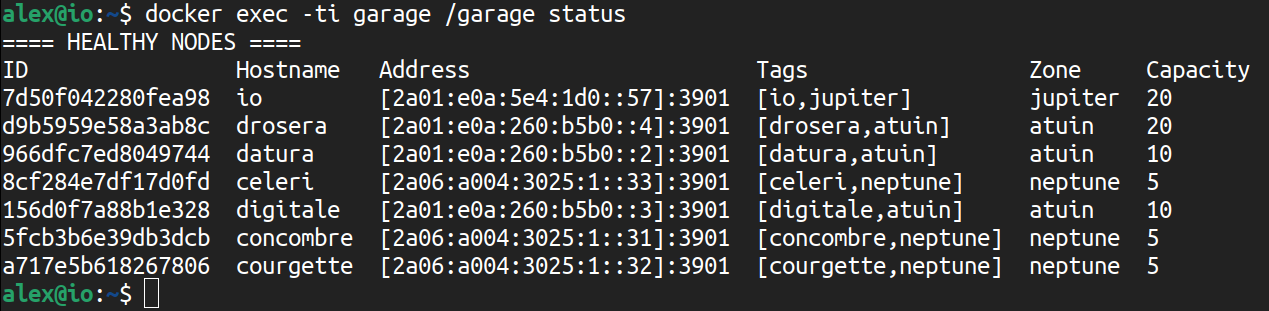
\includegraphics[width=13.25cm]{zones.png}
\end{center}
\end{frame}

\subsection{Comment ça marche ?}
\begin{frame}
\begin{columns}
\column{0.5 \linewidth}
\input{schéma europe}
\column{0.5 \linewidth}
\begin{center}
Chaque objet est dupliqué sur plusieurs zones différentes.\linebreak

\onslide<5->{Lorsqu'un nouvel hébergeur rejoint le réseau, la charge se voit équilibrée.}\linebreak

\onslide<12->{Si une zone devient indisponible, les autres continuent d'assurer le service.}\linebreak
\end{center}
\end{columns}
\end{frame}

\subsection{Financement}
\begin{frame}
\begin{center}
Dans le cadre du programme \textit{Horizon 2021} de l'Union Européenne, nous avons reçu une subvention de la part de l'initiative NGI Pointer\footnote[frame]{Next Generation Internet Program for Open Internet Renovation}.\linebreak

\includegraphics[width=3cm]{drapeau_européen.png}\hspace{1cm}

\includegraphics[width=3cm]{NGI.png}\linebreak

Nous avons ainsi pu financer le développement de Garage pendant 1 an.
\end{center}
\end{frame}

\subsection{Licence}
\begin{frame}
\begin{center}
De par nos valeurs, nous avons attribué la licence AGPL version 3 à Garage, notamment afin qu'il reste parmi les biens communs.\linebreak

\vspace{0.5cm}

\includegraphics[width=5cm]{agpl-v3-logo.png}\linebreak
\end{center}
\end{frame}

\subsection{Langage utilisé}
\begin{frame}
\begin{center}
Nous avons décidé d'écrire Garage à l'aide du langage Rust, afin d'obtenir une compilation vers des binaires natifs et efficaces.\linebreak


\includegraphics[width=3.5cm]{rust-logo.png}\linebreak

Ce choix permet également de bénéficier des avantages reconnus de Rust en termes de sécurité.
\end{center}
\end{frame}

\subsection{Matériel requis}
\begin{frame}
\begin{center}
Garage peut ainsi être performant sur des machines limitées. Les prérequis sont minimes : n'importe quelle machine avec un processeur qui a moins d'une décennie, 1~gigaoctet de mémoire vive, et 16~gigaoctets de stockage suffit.\linebreak

\vspace{1cm}

Cet aspect est déterminant : il permet en effet d'héberger sur du matériel acheté d'occasion, pour réduire l'impact écologique de nos infrastructures.
\end{center}
\end{frame}

\subsection{Performances}
\begin{frame}
\begin{center}
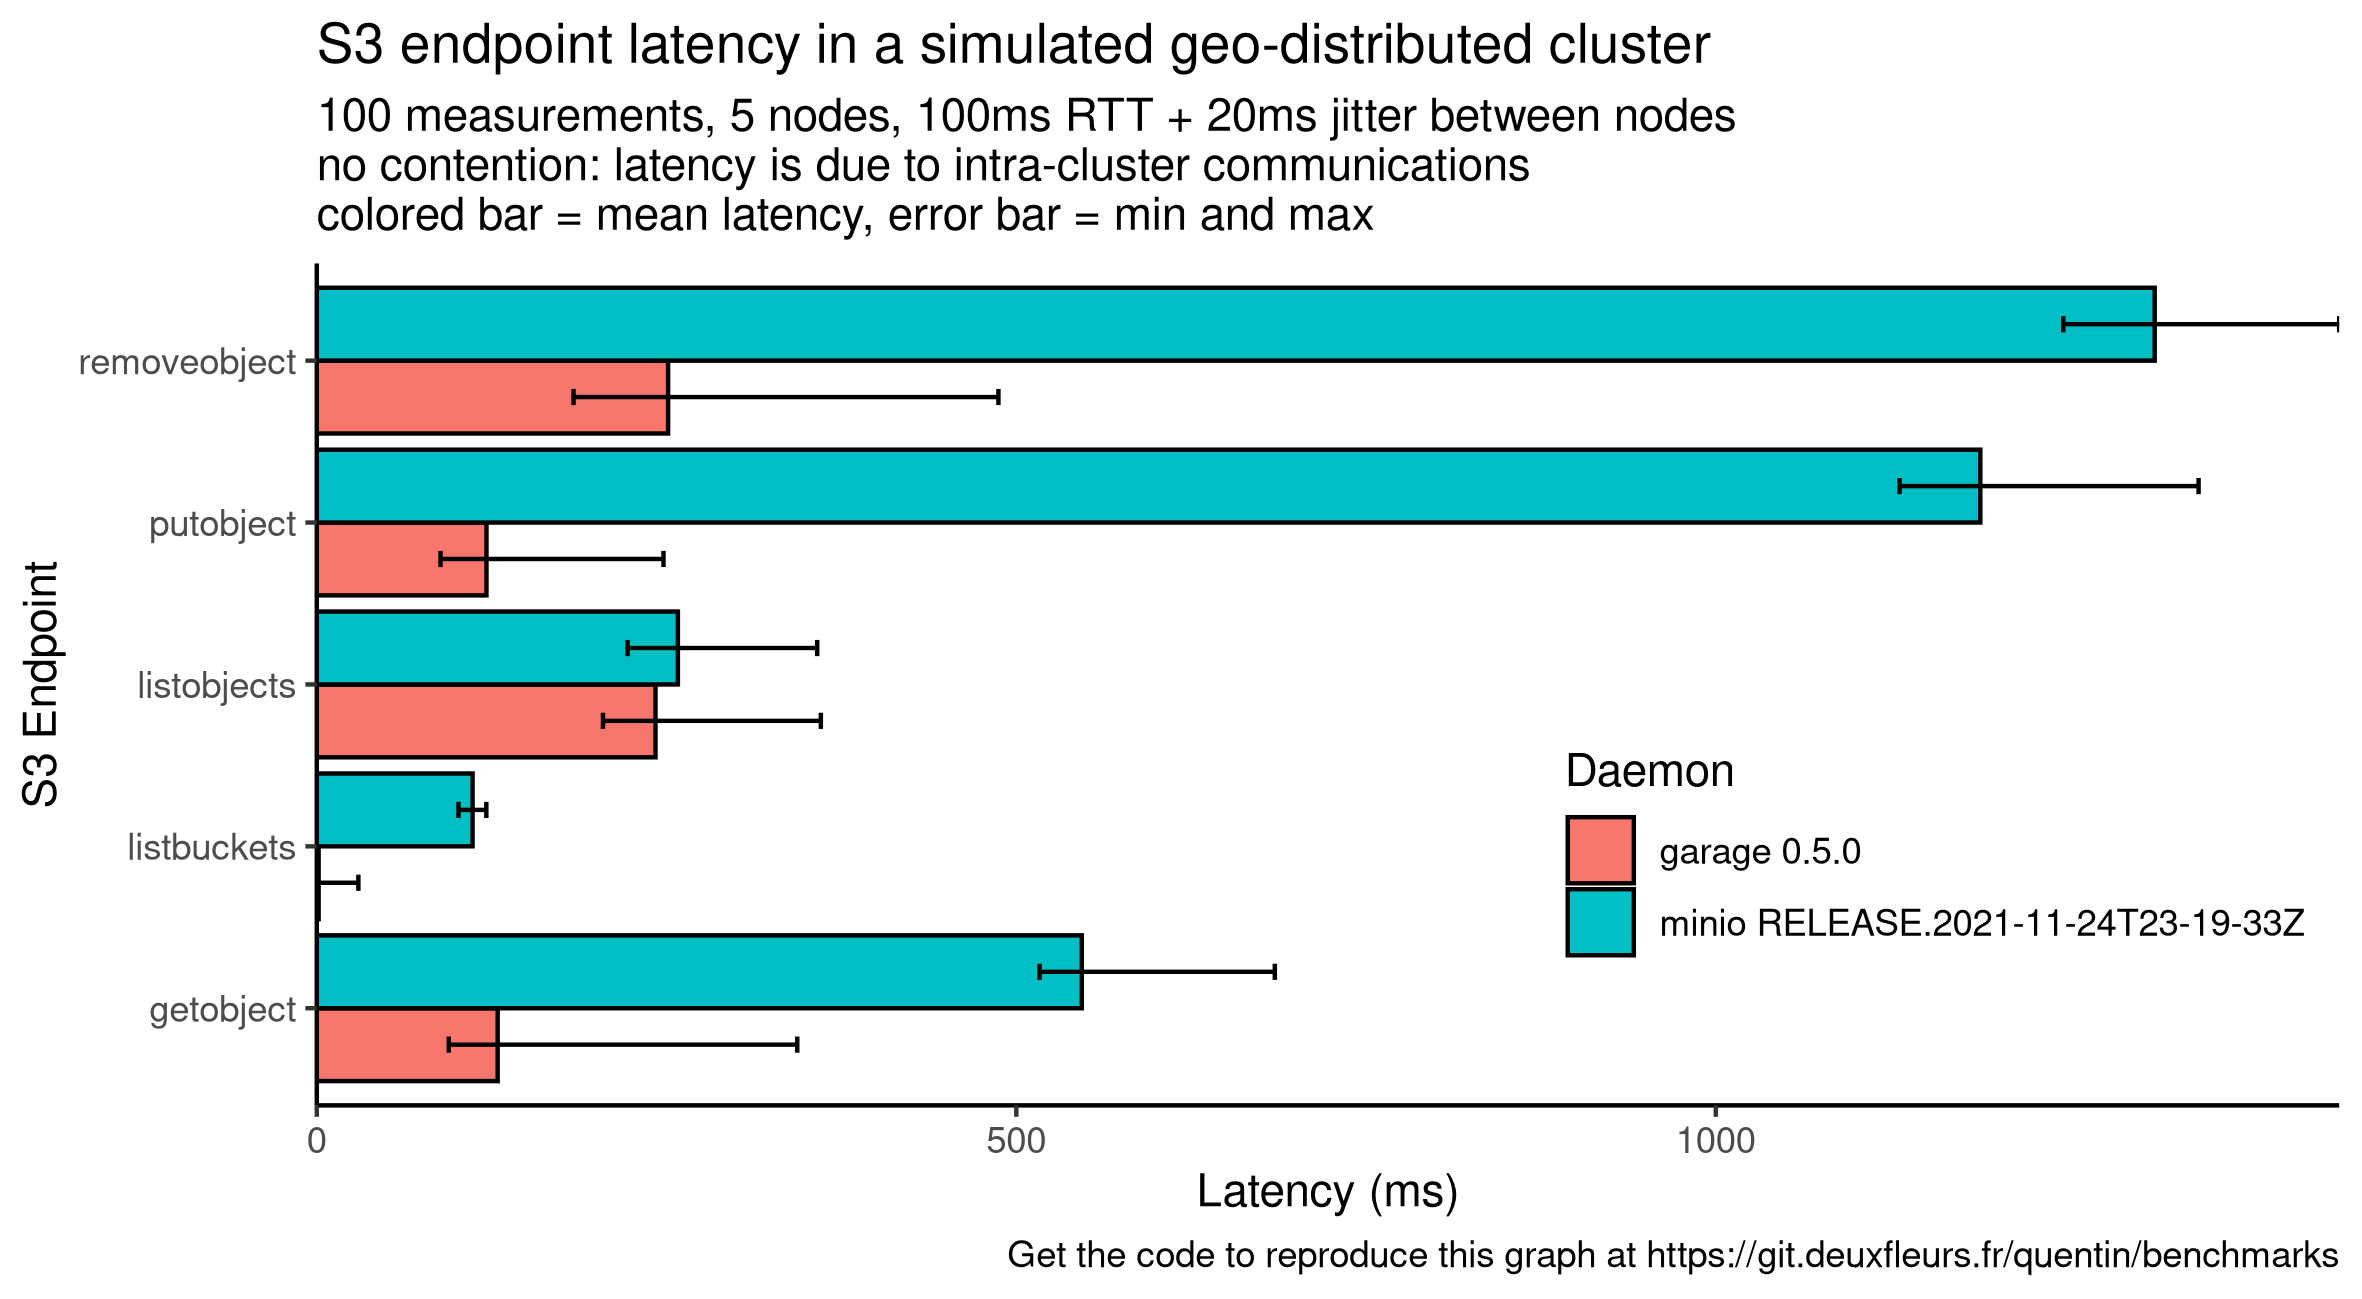
\includegraphics[width=13.25cm]{rpc-amplification.png}
\end{center}
\end{frame}

\begin{frame}
\begin{center}
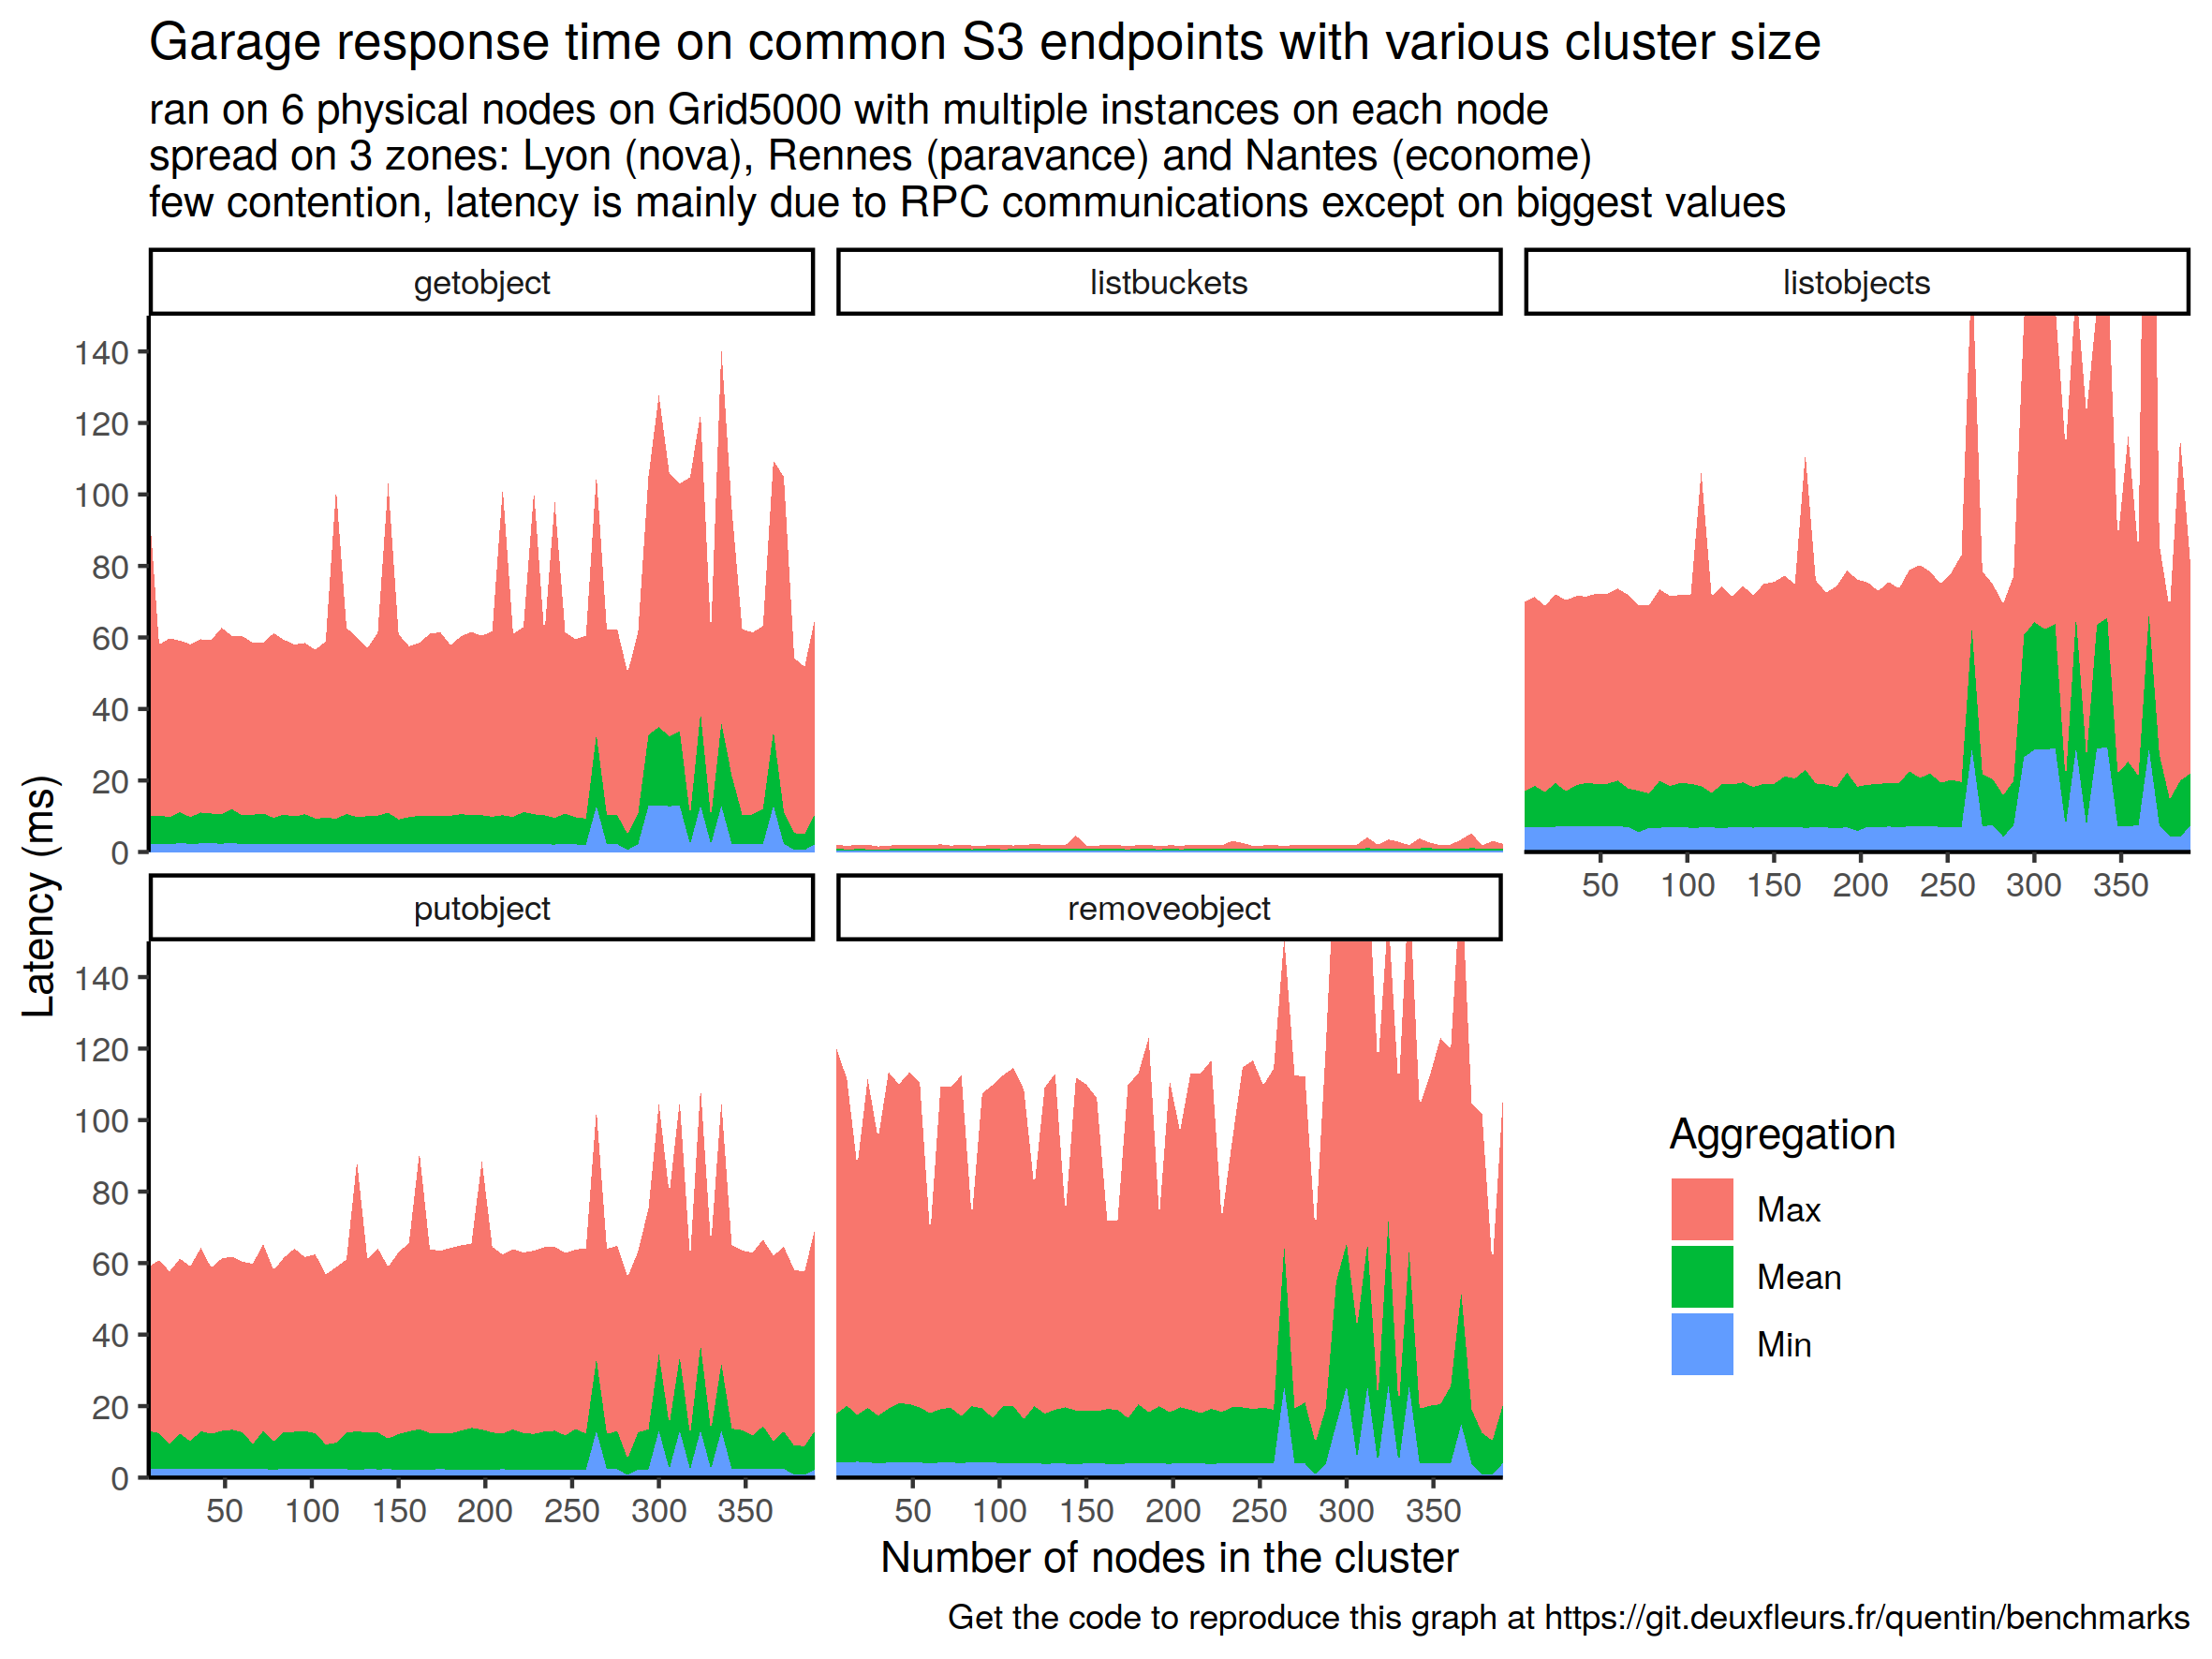
\includegraphics[width=11cm]{rpc-complexity.png}
\end{center}
\end{frame}

\subsection{Services}
\begin{frame}
\begin{center}
Puisqu'il suit le standard S3, beaucoup de services populaires sont par conséquence compatibles avec Garage :\linebreak

\begin{columns}
\column{0.2 \linewidth}
\begin{center}

\includegraphics[width=2.5cm]{nextcloud-logo.png}
\end{center}
\column{0.2 \linewidth}
\begin{center}

\includegraphics[width=2.5cm]{peertube-logo.png}
\end{center}
\column{0.2 \linewidth}
\begin{center}

\includegraphics[width=2.5cm]{matrix-logo.png}
\end{center}
\column{0.2 \linewidth}
\begin{center}

\includegraphics[width=2.5cm]{mastodon-logo.png}
\end{center}
\end{columns}
~\linebreak

Et comme souvent avec S3, on peut assimiler un bucket à un site, et utiliser le serveur pour héberger des sites web statiques.
\end{center}
\end{frame}

\section{Intégration chez Deuxfleurs}
\subsection{Matériel}
\begin{frame}
\begin{center}
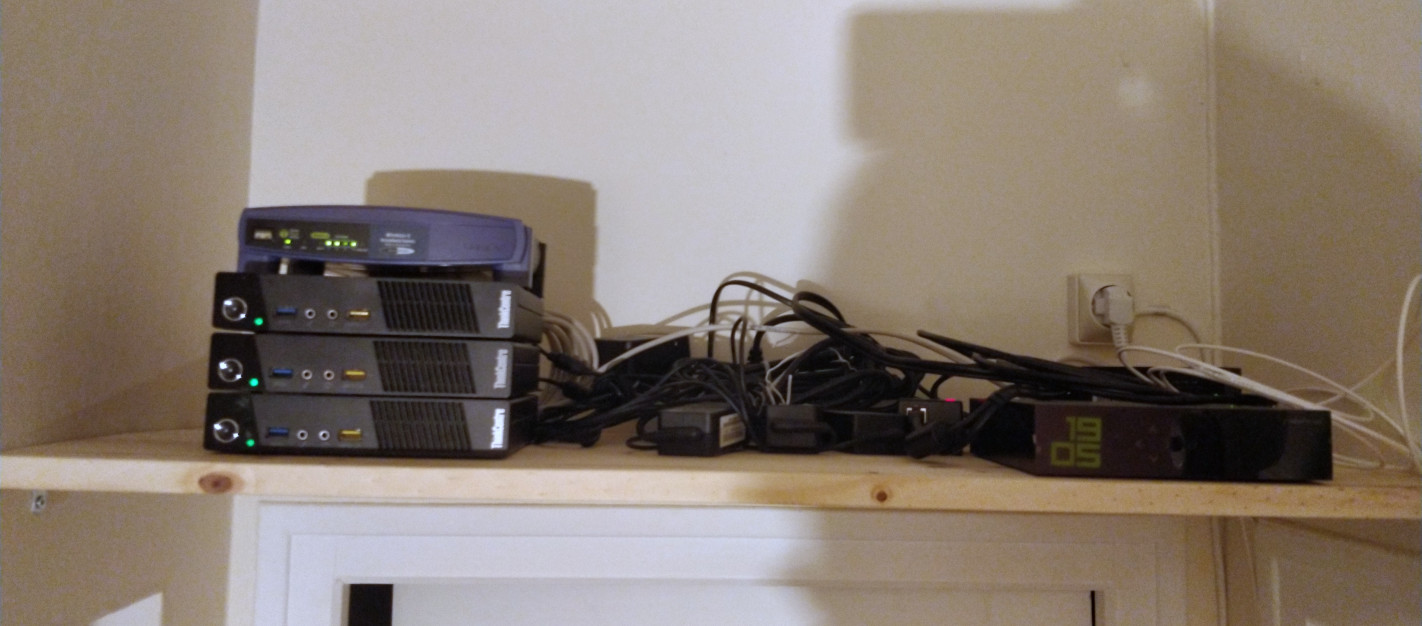
\includegraphics[width=13cm]{neptune.jpg}\linebreak

En pratique, nos serveurs ne sont effectivement que des machines achetées d'occasion (très souvent des anciens ordinateurs destinés à la bureautique en entreprise).
\end{center}
\end{frame}

\subsection{Environnement logiciel}
\begin{frame}
\begin{center}
Pour faciliter la reproduction d'un environnement connu, NixOS est installé sur nos machines.\linebreak

\vspace{1cm}
Pour s’accommoder des réseaux qu'on trouve derrière des routeurs pour particuliers, on s'aide de notre logiciel Diplonat\footnote[frame]{\texttt{https://git.deuxfleurs.fr/Deuxfleurs/diplonat}}.
\end{center}
\end{frame}

\section{Au-delà...}
\subsection{... de Deuxfleurs}
\begin{frame}
\begin{center}
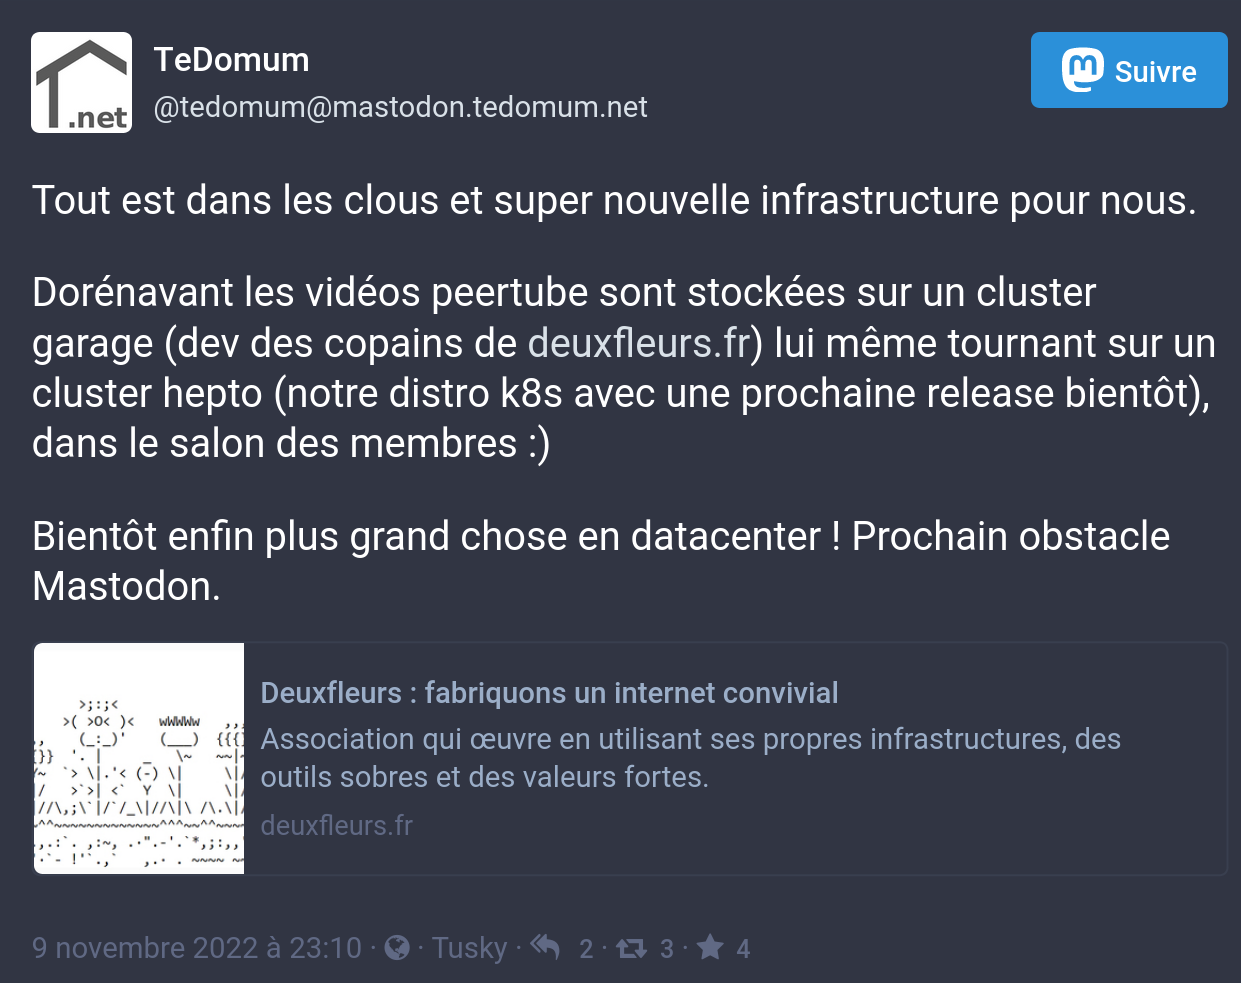
\includegraphics[width=10cm]{tedomum.png}
\end{center}
\end{frame}

\subsection{... de Garage}
\begin{frame}
\begin{center}
Nous avons récemment lancé le développement d'Aérogramme\footnote[frame]{\texttt{https://git.deuxfleurs.fr/Deuxfleurs/aerogramme}}.\linebreak

\vspace{1cm}
Il s'agit d'un serveur de stockage de courriels chiffrés.\linebreak

\vspace{1cm}
Il est conçu pour pouvoir travailler avec Garage.
\end{center}
\end{frame}

\section{Fin}
\subsection{Contacts}
\begin{frame}
\begin{center}
\begin{tikzpicture}
\node (ronce) {
\includegraphics[width=0.95\textwidth]{ronce.jpg}};
\node[white] at (-5.1,3.6) {Intéressé(e) ?};
\node[white, align=center] at (4.2,-2.6) {Contactez-nous !\\\texttt{coucou@deuxfleurs.fr}\\\texttt{\#forum:deuxfleurs.fr}};
\end{tikzpicture}
\end{center}
\end{frame}
\end{document}

